\documentclass[a4paper,10pt]{scrartcl}
\usepackage[backend=biber,bibencoding=utf-8]{biblatex}

\usepackage{praeambel}

%%% Eigene Daten: Beginn
\title{Entwicklungsarbeit}
\newcommand\authorA{Sebastian Schramm}
\newcommand\matrikelnrA{-}
\newcommand\modul{Programmieren 1}
\newcommand\pruefer{-}
\date{\today}
%%% Eigene Daten: Ende

\begin{document}
\selectlanguage{ngerman}
\begin{titlepage}
  \pagestyle{empty}
  \centering

  \vspace*{0.5cm}
  \begin{otherlanguage*}{ngerman}
    \begin{sffamily} {
        \Large
        Hochschule -\\[1em]
        Fakultät IV -- Technische Informatik\\[0.1em]
        Modul: \modul\\[0.1em]
        Prüfer: \pruefer\\[0.1em]
        Semester: \semester\\[0.1em]
      }
    \end{sffamily}
  \end{otherlanguage*}

  \vspace*{3cm}

  \begin{sffamily}
    \huge \bfseries
    \makeatletter
    \@title
    \makeatother
    \\
  \end{sffamily}

  \vspace*{1cm}

  \begin{otherlanguage*}{ngerman}
    
    \vspace*{3cm}
    
    von\\[0.75em]
    {
      \large
      \textbf{\authorA}\quad Matrikel-Nr. \matrikelnrA\\
      %\textbf{\authorB}\quad Matrikel-Nr. \matrikelnrB

      \vspace*{2cm}
      \makeatletter
      \@date
      \makeatother
    }
    \vfill
  \end{otherlanguage*}
\end{titlepage}

\tableofcontents

\newpage

%%% Protokoll: Beginn

\section{Kapitel 1}
\subsection{Aufgabenstellung}
Wir sollen ein Programm schreiben welches den Text "Dear Prudence\dq \space in der Konsole ausgibt. 
Um uns mit Java vertraut zu machen, sollten wir das erste Programm in der Kommandozeile schreiben.
Anschlie\ss end mit Javac Kompilieren und mit Java ausführen. Danach öffnen wir unsere IDE, erstellen
ein neues Projekt und schreib das selbe Programm diesmal in der IDE.

\subsection{Anforderungsdefinition}
\begin{enumerate}
	\item Das Programm soll "Dear Prudence\dq \space auf der Konsole ausgeben.
\end{enumerate}

\subsection{Entwurf}
\section{Kapitel 1}
\subsection{Aufgabenstellung}
Wir sollen ein Programm schreiben welches den Text "Dear Prudence\dq \space in der Konsole ausgibt. 
Um uns mit Java vertraut zu machen, sollten wir das erste Programm in der Kommandozeile schreiben.
Anschlie\ss end mit Javac Kompilieren und mit Java ausführen. Danach öffnen wir unsere IDE, erstellen
ein neues Projekt und schreib das selbe Programm diesmal in der IDE.

\subsection{Anforderungsdefinition}
\begin{enumerate}
	\item Das Programm soll "Dear Prudence\dq \space auf der Konsole ausgeben.
\end{enumerate}

\subsection{Entwurf}
\section{Kapitel 1}
\subsection{Aufgabenstellung}
Wir sollen ein Programm schreiben welches den Text "Dear Prudence\dq \space in der Konsole ausgibt. 
Um uns mit Java vertraut zu machen, sollten wir das erste Programm in der Kommandozeile schreiben.
Anschlie\ss end mit Javac Kompilieren und mit Java ausführen. Danach öffnen wir unsere IDE, erstellen
ein neues Projekt und schreib das selbe Programm diesmal in der IDE.

\subsection{Anforderungsdefinition}
\begin{enumerate}
	\item Das Programm soll "Dear Prudence\dq \space auf der Konsole ausgeben.
\end{enumerate}

\subsection{Entwurf}
\input{uml/chapter_01_part2.tex}

\subsection{Quellcode}
\subsubsection{Main.java}
\lstinputlisting[language = Java , frame = trBL , firstnumber = last , escapeinside={(*@}{@*)}]{../chapter_01/src/chapter_01/Main.java}

\subsection{Testdokumentation}
Wenn das Programm gestartet wird, sollte "Dear Prudence\dq \space auf der Konsole ausgegeben werde.
Dies war der fall.

\subsection{Benutzungshinweise}
Navigieren Sie in der Kommandozeile zum dem Ordner, wo sich die Java Datei befindet.
Danach führen sie "javac Main.java\dq \space auf. Jetzt können Sie das Programm mit "java main\dq \space
 starten. In der Konsole sollte nun "Dear Prudence\dq \space angezeigt werden.

\subsection{Anwendungsbeispiel}
Nach dem Aufruf von java Main, sollten wir folgendes sehen:
\begin{lstlisting}[frame = trBL , escapeinside={(*@}{@*)}]
[sebastian@laptop bin]$ java Main 
Dear Prudence
[sebastian@laptop bin]$ 
\end{lstlisting}

\subsection{Quellcode}
\subsubsection{Main.java}
\lstinputlisting[language = Java , frame = trBL , firstnumber = last , escapeinside={(*@}{@*)}]{../chapter_01/src/chapter_01/Main.java}

\subsection{Testdokumentation}
Wenn das Programm gestartet wird, sollte "Dear Prudence\dq \space auf der Konsole ausgegeben werde.
Dies war der fall.

\subsection{Benutzungshinweise}
Navigieren Sie in der Kommandozeile zum dem Ordner, wo sich die Java Datei befindet.
Danach führen sie "javac Main.java\dq \space auf. Jetzt können Sie das Programm mit "java main\dq \space
 starten. In der Konsole sollte nun "Dear Prudence\dq \space angezeigt werden.

\subsection{Anwendungsbeispiel}
Nach dem Aufruf von java Main, sollten wir folgendes sehen:
\begin{lstlisting}[frame = trBL , escapeinside={(*@}{@*)}]
[sebastian@laptop bin]$ java Main 
Dear Prudence
[sebastian@laptop bin]$ 
\end{lstlisting}

\subsection{Quellcode}
\subsubsection{Main.java}
\lstinputlisting[language = Java , frame = trBL , firstnumber = last , escapeinside={(*@}{@*)}]{../chapter_01/src/chapter_01/Main.java}

\subsection{Testdokumentation}
Wenn das Programm gestartet wird, sollte "Dear Prudence\dq \space auf der Konsole ausgegeben werde.
Dies war der fall.

\subsection{Benutzungshinweise}
Navigieren Sie in der Kommandozeile zum dem Ordner, wo sich die Java Datei befindet.
Danach führen sie "javac Main.java\dq \space auf. Jetzt können Sie das Programm mit "java main\dq \space
 starten. In der Konsole sollte nun "Dear Prudence\dq \space angezeigt werden.

\subsection{Anwendungsbeispiel}
Nach dem Aufruf von java Main, sollten wir folgendes sehen:
\begin{lstlisting}[frame = trBL , escapeinside={(*@}{@*)}]
[sebastian@laptop bin]$ java Main 
Dear Prudence
[sebastian@laptop bin]$ 
\end{lstlisting}
\section{Kapitel 3}
\subsection{Teilaufgabe 1}
\subsubsection{Aufgabenstellung}
In der ersten Teilaufgabe sollten wir uns mit der Typkonvertierung befassen. Welches alle
primitive Datentypen erweiternd und einschränkend Konvertiert.

\subsubsection{Anforderungsdefinition}
\begin{enumerate}
	\item Zu jedem Primitiven Datentypen eine erweiternde und einschränkende Konvertierung
	durchführen.
\end{enumerate}

\subsubsection{Entwurf}
\section{Kapitel 3}
\subsection{Teilaufgabe 1}
\subsubsection{Aufgabenstellung}
In der ersten Teilaufgabe sollten wir uns mit der Typkonvertierung befassen. Welches alle
primitive Datentypen erweiternd und einschränkend Konvertiert.

\subsubsection{Anforderungsdefinition}
\begin{enumerate}
	\item Zu jedem Primitiven Datentypen eine erweiternde und einschränkende Konvertierung
	durchführen.
\end{enumerate}

\subsubsection{Entwurf}
\section{Kapitel 3}
\subsection{Teilaufgabe 1}
\subsubsection{Aufgabenstellung}
In der ersten Teilaufgabe sollten wir uns mit der Typkonvertierung befassen. Welches alle
primitive Datentypen erweiternd und einschränkend Konvertiert.

\subsubsection{Anforderungsdefinition}
\begin{enumerate}
	\item Zu jedem Primitiven Datentypen eine erweiternde und einschränkende Konvertierung
	durchführen.
\end{enumerate}

\subsubsection{Entwurf}
\input{uml/chapter_03_part1.tex}

\subsubsection{Quelltext}
\paragraph{Typkonvertierungen.java}\
\lstinputlisting[language = Java , frame = trBL , escapeinside={(*@}{@*)}]{../chapter_03/src/chapter_03/Typkonvertierungen.java}

\subsubsection{Testdokumentation}

\subsubsection{Benutzungshinweise}
Keine Besonderen Benutzungshinweise.
Man navigiere zu dem Ordner von sich die Compilierte Datei mit dem Namen "Typkonvertierungen.class"
\space befindet und führt anschlie\ss end java Typkonvertierungen aus.

\subsubsection{Anwendungsbeispiel}
Nach dem man das Programm gestartet hat, sollte folgende Ausgabe erscheinen:
\begin{lstlisting}[frame = trBL , escapeinside={(*@}{@*)}]
[sebastian@laptop bin]$ java Typkonvertierungen 
---------------------
Byte erweiternd
Byte   -128
Short  -128
Int    -128
Long   -128
FLoat  -128.0
Bouble -128.0

Char   タ
---------------------
Short einschraenkend
Short  34
Byte   34
Short erweiternd
Short  34
Int    34
Long   34
FLoat  34.0
Bouble 34.0

Char   "
---------------------
Int einschraenkend
Int    98987
Short  -32085
Byte   -85
Int erweiternd
Int    98987
Long   98987
FLoat  98987.0
Bouble 98987.0

Char   芫
---------------------
Long einschraenkend
Long   987987987
Int    987987987
Short  -32749
Byte   19
Long erweiternd
Long   987987987
FLoat  9.8798797E8
Bouble 9.87987987E8

Char   耓
---------------------
Char einschraenkend
Char   a
Long   97
Int    97
Short  97
Byte   97
Char erweiternd
Char   a
Long   97
FLoat  97.0
Bouble 97.0
---------------------
Float einschraenkend
FLoat  15.0
Long   15
Int    15
Short  15
Byte   15
Float erweiternd
FLoat  15.0
Bouble 15.0

Char   
---------------------
Double einschraenkend
Bouble 1.7976931348623157E308
FLoat  Infinity
Long   9223372036854775807
Int    2147483647
Short  -1
Byte   -1

Char   ￿
---------------------
[sebastian@laptop bin]$ 
\end{lstlisting}


\subsubsection{Quelltext}
\paragraph{Typkonvertierungen.java}\
\lstinputlisting[language = Java , frame = trBL , escapeinside={(*@}{@*)}]{../chapter_03/src/chapter_03/Typkonvertierungen.java}

\subsubsection{Testdokumentation}

\subsubsection{Benutzungshinweise}
Keine Besonderen Benutzungshinweise.
Man navigiere zu dem Ordner von sich die Compilierte Datei mit dem Namen "Typkonvertierungen.class"
\space befindet und führt anschlie\ss end java Typkonvertierungen aus.

\subsubsection{Anwendungsbeispiel}
Nach dem man das Programm gestartet hat, sollte folgende Ausgabe erscheinen:
\begin{lstlisting}[frame = trBL , escapeinside={(*@}{@*)}]
[sebastian@laptop bin]$ java Typkonvertierungen 
---------------------
Byte erweiternd
Byte   -128
Short  -128
Int    -128
Long   -128
FLoat  -128.0
Bouble -128.0

Char   タ
---------------------
Short einschraenkend
Short  34
Byte   34
Short erweiternd
Short  34
Int    34
Long   34
FLoat  34.0
Bouble 34.0

Char   "
---------------------
Int einschraenkend
Int    98987
Short  -32085
Byte   -85
Int erweiternd
Int    98987
Long   98987
FLoat  98987.0
Bouble 98987.0

Char   芫
---------------------
Long einschraenkend
Long   987987987
Int    987987987
Short  -32749
Byte   19
Long erweiternd
Long   987987987
FLoat  9.8798797E8
Bouble 9.87987987E8

Char   耓
---------------------
Char einschraenkend
Char   a
Long   97
Int    97
Short  97
Byte   97
Char erweiternd
Char   a
Long   97
FLoat  97.0
Bouble 97.0
---------------------
Float einschraenkend
FLoat  15.0
Long   15
Int    15
Short  15
Byte   15
Float erweiternd
FLoat  15.0
Bouble 15.0

Char   
---------------------
Double einschraenkend
Bouble 1.7976931348623157E308
FLoat  Infinity
Long   9223372036854775807
Int    2147483647
Short  -1
Byte   -1

Char   ￿
---------------------
[sebastian@laptop bin]$ 
\end{lstlisting}


\subsubsection{Quelltext}
\paragraph{Typkonvertierungen.java}\
\lstinputlisting[language = Java , frame = trBL , escapeinside={(*@}{@*)}]{../chapter_03/src/chapter_03/Typkonvertierungen.java}

\subsubsection{Testdokumentation}

\subsubsection{Benutzungshinweise}
Keine Besonderen Benutzungshinweise.
Man navigiere zu dem Ordner von sich die Compilierte Datei mit dem Namen "Typkonvertierungen.class"
\space befindet und führt anschlie\ss end java Typkonvertierungen aus.

\subsubsection{Anwendungsbeispiel}
Nach dem man das Programm gestartet hat, sollte folgende Ausgabe erscheinen:
\begin{lstlisting}[frame = trBL , escapeinside={(*@}{@*)}]
[sebastian@laptop bin]$ java Typkonvertierungen 
---------------------
Byte erweiternd
Byte   -128
Short  -128
Int    -128
Long   -128
FLoat  -128.0
Bouble -128.0

Char   タ
---------------------
Short einschraenkend
Short  34
Byte   34
Short erweiternd
Short  34
Int    34
Long   34
FLoat  34.0
Bouble 34.0

Char   "
---------------------
Int einschraenkend
Int    98987
Short  -32085
Byte   -85
Int erweiternd
Int    98987
Long   98987
FLoat  98987.0
Bouble 98987.0

Char   芫
---------------------
Long einschraenkend
Long   987987987
Int    987987987
Short  -32749
Byte   19
Long erweiternd
Long   987987987
FLoat  9.8798797E8
Bouble 9.87987987E8

Char   耓
---------------------
Char einschraenkend
Char   a
Long   97
Int    97
Short  97
Byte   97
Char erweiternd
Char   a
Long   97
FLoat  97.0
Bouble 97.0
---------------------
Float einschraenkend
FLoat  15.0
Long   15
Int    15
Short  15
Byte   15
Float erweiternd
FLoat  15.0
Bouble 15.0

Char   
---------------------
Double einschraenkend
Bouble 1.7976931348623157E308
FLoat  Infinity
Long   9223372036854775807
Int    2147483647
Short  -1
Byte   -1

Char   ￿
---------------------
[sebastian@laptop bin]$ 
\end{lstlisting}

% generated by Plantuml 1.2018.13      
\definecolor{plantucolor0000}{RGB}{0,0,0}
\definecolor{plantucolor0001}{RGB}{254,254,206}
\definecolor{plantucolor0002}{RGB}{168,0,54}
\begin{tikzpicture}[yscale=-1
,pstyle0/.style={fill=black,line width=1.0pt}
,pstyle1/.style={color=plantucolor0002,fill=plantucolor0001,line width=1.5pt}
,pstyle3/.style={color=plantucolor0002,line width=1.5pt}
,pstyle4/.style={color=plantucolor0002,fill=plantucolor0002,line width=1.0pt}
]
\draw[pstyle0] (99.5412pt,20pt) ellipse (10pt and 10pt);
\draw[pstyle1] (18.5775pt,66.9844pt) arc (180:270:16.9844pt) -- (35.5619pt,50pt) -- (163.5204pt,50pt) arc (270:360:16.9844pt) -- (180.5048pt,66.9844pt) -- (180.5048pt,66.9844pt) arc (0:90:16.9844pt) -- (163.5204pt,83.9688pt) -- (35.5619pt,83.9688pt) arc (90:180:16.9844pt) -- (18.5775pt,66.9844pt) -- cycle;
\node at (50pt,60pt)[below right,color=black]{print Byte min max};
\draw[pstyle1] (15.1634pt,120.9531pt) arc (180:270:16.9844pt) -- (32.1478pt,103.9688pt) -- (166.9346pt,103.9688pt) arc (270:360:16.9844pt) -- (183.919pt,120.9531pt) -- (183.919pt,120.9531pt) arc (0:90:16.9844pt) -- (166.9346pt,137.9375pt) -- (32.1478pt,137.9375pt) arc (90:180:16.9844pt) -- (15.1634pt,120.9531pt) -- cycle;
\node at (50pt,113.9688pt)[below right,color=black]{print Short min max};
\draw[pstyle1] (24.4139pt,174.9219pt) arc (180:270:16.9844pt) -- (41.3983pt,157.9375pt) -- (157.6841pt,157.9375pt) arc (270:360:16.9844pt) -- (174.6684pt,174.9219pt) -- (174.6684pt,174.9219pt) arc (0:90:16.9844pt) -- (157.6841pt,191.9063pt) -- (41.3983pt,191.9063pt) arc (90:180:16.9844pt) -- (24.4139pt,174.9219pt) -- cycle;
\node at (50pt,167.9375pt)[below right,color=black]{print Int min max};
\draw[pstyle1] (16.8831pt,228.8906pt) arc (180:270:16.9844pt) -- (33.8675pt,211.9063pt) -- (165.2149pt,211.9063pt) arc (270:360:16.9844pt) -- (182.1992pt,228.8906pt) -- (182.1992pt,228.8906pt) arc (0:90:16.9844pt) -- (165.2149pt,245.875pt) -- (33.8675pt,245.875pt) arc (90:180:16.9844pt) -- (16.8831pt,228.8906pt) -- cycle;
\node at (50pt,221.9063pt)[below right,color=black]{print Long min max};
\draw[pstyle1] (16.8794pt,282.8594pt) arc (180:270:16.9844pt) -- (33.8638pt,265.875pt) -- (165.2186pt,265.875pt) arc (270:360:16.9844pt) -- (182.203pt,282.8594pt) -- (182.203pt,282.8594pt) arc (0:90:16.9844pt) -- (165.2186pt,299.8438pt) -- (33.8638pt,299.8438pt) arc (90:180:16.9844pt) -- (16.8794pt,282.8594pt) -- cycle;
\node at (50pt,275.875pt)[below right,color=black]{print Char min max};
\draw[pstyle1] (10pt,336.8281pt) arc (180:270:16.9844pt) -- (26.9844pt,319.8438pt) -- (172.098pt,319.8438pt) arc (270:360:16.9844pt) -- (189.0824pt,336.8281pt) -- (189.0824pt,336.8281pt) arc (0:90:16.9844pt) -- (172.098pt,353.8125pt) -- (26.9844pt,353.8125pt) arc (90:180:16.9844pt) -- (10pt,336.8281pt) -- cycle;
\node at (50pt,329.8438pt)[below right,color=black]{print Double min max};
\draw[pstyle1] (16.3831pt,390.7969pt) arc (180:270:16.9844pt) -- (33.3675pt,373.8125pt) -- (165.7149pt,373.8125pt) arc (270:360:16.9844pt) -- (182.6992pt,390.7969pt) -- (182.6992pt,390.7969pt) arc (0:90:16.9844pt) -- (165.7149pt,407.7813pt) -- (33.3675pt,407.7813pt) arc (90:180:16.9844pt) -- (16.3831pt,390.7969pt) -- cycle;
\node at (50pt,383.8125pt)[below right,color=black]{print Float min max};
\draw[color=black,line width=1.0pt] (99.5412pt,437.7813pt) ellipse (10pt and 10pt);
\draw[pstyle0] (100.0412pt,438.2813pt) ellipse (6pt and 6pt);
\draw[pstyle3] (99.5412pt,30pt) -- (99.5412pt,50pt);
\draw[pstyle4] (95.5412pt,40pt) -- (99.5412pt,50pt) -- (103.5412pt,40pt) -- (99.5412pt,44pt) -- cycle;
\draw[pstyle3] (99.5412pt,83.9688pt) -- (99.5412pt,103.9688pt);
\draw[pstyle4] (95.5412pt,93.9688pt) -- (99.5412pt,103.9688pt) -- (103.5412pt,93.9688pt) -- (99.5412pt,97.9688pt) -- cycle;
\draw[pstyle3] (99.5412pt,137.9375pt) -- (99.5412pt,157.9375pt);
\draw[pstyle4] (95.5412pt,147.9375pt) -- (99.5412pt,157.9375pt) -- (103.5412pt,147.9375pt) -- (99.5412pt,151.9375pt) -- cycle;
\draw[pstyle3] (99.5412pt,191.9063pt) -- (99.5412pt,211.9063pt);
\draw[pstyle4] (95.5412pt,201.9063pt) -- (99.5412pt,211.9063pt) -- (103.5412pt,201.9063pt) -- (99.5412pt,205.9063pt) -- cycle;
\draw[pstyle3] (99.5412pt,245.875pt) -- (99.5412pt,265.875pt);
\draw[pstyle4] (95.5412pt,255.875pt) -- (99.5412pt,265.875pt) -- (103.5412pt,255.875pt) -- (99.5412pt,259.875pt) -- cycle;
\draw[pstyle3] (99.5412pt,299.8438pt) -- (99.5412pt,319.8438pt);
\draw[pstyle4] (95.5412pt,309.8438pt) -- (99.5412pt,319.8438pt) -- (103.5412pt,309.8438pt) -- (99.5412pt,313.8438pt) -- cycle;
\draw[pstyle3] (99.5412pt,353.8125pt) -- (99.5412pt,373.8125pt);
\draw[pstyle4] (95.5412pt,363.8125pt) -- (99.5412pt,373.8125pt) -- (103.5412pt,363.8125pt) -- (99.5412pt,367.8125pt) -- cycle;
\draw[pstyle3] (99.5412pt,407.7813pt) -- (99.5412pt,427.7813pt);
\draw[pstyle4] (95.5412pt,417.7813pt) -- (99.5412pt,427.7813pt) -- (103.5412pt,417.7813pt) -- (99.5412pt,421.7813pt) -- cycle;
\end{tikzpicture}

\section{Kapitel 4}
\subsection{Teilaufgabe 1}
\subsubsection{Aufgabenstellung}
Wir sollen ein Programm schreiben welches Prüft ob zwei Referenzen gleich sind.

\subsubsection{Anforderungsdefinition}
\begin{enumerate}
	\item Prüfe ob zwei Referenzen gleich sind.
\end{enumerate}

\subsubsection{Entwurf}
\section{Kapitel 4}
\subsection{Teilaufgabe 1}
\subsubsection{Aufgabenstellung}
Wir sollen ein Programm schreiben welches Prüft ob zwei Referenzen gleich sind.

\subsubsection{Anforderungsdefinition}
\begin{enumerate}
	\item Prüfe ob zwei Referenzen gleich sind.
\end{enumerate}

\subsubsection{Entwurf}
\section{Kapitel 4}
\subsection{Teilaufgabe 1}
\subsubsection{Aufgabenstellung}
Wir sollen ein Programm schreiben welches Prüft ob zwei Referenzen gleich sind.

\subsubsection{Anforderungsdefinition}
\begin{enumerate}
	\item Prüfe ob zwei Referenzen gleich sind.
\end{enumerate}

\subsubsection{Entwurf}
\input{uml/chapter_04_part1.tex}

\subsubsection{Quellcode}
\paragraph{Referenzen.java}\
\lstinputlisting[language = Java , frame = trBL , escapeinside={(*@}{@*)}]{../chapter_04/src/chapter_04/Referenzen.java}
\paragraph{Punkt.java}\
\lstinputlisting[language = Java , frame = trBL , escapeinside={(*@}{@*)}]{../chapter_04/src/chapter_04/Punkt.java}

\subsubsection{Testdokumentation}

\subsubsection{Benutzungshinweise}
Navigieren Sie in der Kommandozeile zum dem Ordner, wo sich die Java Datei befindet.
Danach führen sie "javac Referenzen.java\dq \space auf. Jetzt können Sie das Programm mit
"java Referenzen\dq \space starten.

\subsubsection{Anwendungsbeispiel}
Nach dem Aufruf von java Referenzen, sollten wir nun folgendes sehen:
\begin{lstlisting}[frame = trBL , escapeinside={(*@}{@*)}]
[sebastian@laptop bin]$ java Referenzen 
Ist ungleich
Ist ungleich
Ist gleich
[sebastian@laptop bin]$  
\end{lstlisting}


\subsubsection{Quellcode}
\paragraph{Referenzen.java}\
\lstinputlisting[language = Java , frame = trBL , escapeinside={(*@}{@*)}]{../chapter_04/src/chapter_04/Referenzen.java}
\paragraph{Punkt.java}\
\lstinputlisting[language = Java , frame = trBL , escapeinside={(*@}{@*)}]{../chapter_04/src/chapter_04/Punkt.java}

\subsubsection{Testdokumentation}

\subsubsection{Benutzungshinweise}
Navigieren Sie in der Kommandozeile zum dem Ordner, wo sich die Java Datei befindet.
Danach führen sie "javac Referenzen.java\dq \space auf. Jetzt können Sie das Programm mit
"java Referenzen\dq \space starten.

\subsubsection{Anwendungsbeispiel}
Nach dem Aufruf von java Referenzen, sollten wir nun folgendes sehen:
\begin{lstlisting}[frame = trBL , escapeinside={(*@}{@*)}]
[sebastian@laptop bin]$ java Referenzen 
Ist ungleich
Ist ungleich
Ist gleich
[sebastian@laptop bin]$  
\end{lstlisting}


\subsubsection{Quellcode}
\paragraph{Referenzen.java}\
\lstinputlisting[language = Java , frame = trBL , escapeinside={(*@}{@*)}]{../chapter_04/src/chapter_04/Referenzen.java}
\paragraph{Punkt.java}\
\lstinputlisting[language = Java , frame = trBL , escapeinside={(*@}{@*)}]{../chapter_04/src/chapter_04/Punkt.java}

\subsubsection{Testdokumentation}

\subsubsection{Benutzungshinweise}
Navigieren Sie in der Kommandozeile zum dem Ordner, wo sich die Java Datei befindet.
Danach führen sie "javac Referenzen.java\dq \space auf. Jetzt können Sie das Programm mit
"java Referenzen\dq \space starten.

\subsubsection{Anwendungsbeispiel}
Nach dem Aufruf von java Referenzen, sollten wir nun folgendes sehen:
\begin{lstlisting}[frame = trBL , escapeinside={(*@}{@*)}]
[sebastian@laptop bin]$ java Referenzen 
Ist ungleich
Ist ungleich
Ist gleich
[sebastian@laptop bin]$  
\end{lstlisting}

\subsection{Teilaufgabe 2}
\subsubsection{Aufgabenstellung}
Wir sollen ein Programm schreiben welches welches 2 nxn Matrizen miteinander Addieren und Multiplizieren kann.

\subsubsection{Anforderungsdefinition}
\begin{enumerate}
	\item Addiere zwei nxn Matrizen.
	\item Multipliziere zwei nxn Matrizen.
\end{enumerate}

\subsubsection{Entwurf}
\subsection{Teilaufgabe 2}
\subsubsection{Aufgabenstellung}
Wir sollen ein Programm schreiben welches welches 2 nxn Matrizen miteinander Addieren und Multiplizieren kann.

\subsubsection{Anforderungsdefinition}
\begin{enumerate}
	\item Addiere zwei nxn Matrizen.
	\item Multipliziere zwei nxn Matrizen.
\end{enumerate}

\subsubsection{Entwurf}
\subsection{Teilaufgabe 2}
\subsubsection{Aufgabenstellung}
Wir sollen ein Programm schreiben welches welches 2 nxn Matrizen miteinander Addieren und Multiplizieren kann.

\subsubsection{Anforderungsdefinition}
\begin{enumerate}
	\item Addiere zwei nxn Matrizen.
	\item Multipliziere zwei nxn Matrizen.
\end{enumerate}

\subsubsection{Entwurf}
\input{uml/chapter_04_part2.tex}

\subsubsection{Quellcode}
\paragraph{Matrizen.java}\
\lstinputlisting[language = Java , frame = trBL , escapeinside={(*@}{@*)}]{../chapter_04/src/chapter_04/Matrizen.java}

\subsubsection{Testdokumentation}

\subsubsection{Benutzungshinweise}
Navigieren Sie in der Kommandozeile zum dem Ordner, wo sich die Java Datei befindet.
Danach führen sie "javac Matrizen.java\dq \space auf. Jetzt können Sie das Programm mit
"java Matrizen\dq \space starten. Nach dem das Programm gestartet ist, können Sie die
grö\ss e der Matrix angeben.

\subsubsection{Anwendungsbeispiel}
Nach dem Aufruf von java Matrizen, sollten wir nun folgendes sehen:
\begin{lstlisting}[frame = trBL , escapeinside={(*@}{@*)}]
[sebastian@laptop bin]$ java Matrizen
Matrix A:
70	50	
16	52	

Matrix B:
80	75	
11	33	

Addition von A und B:
150	125	
27	85	

Multiplikation von A und B:
For Schleife
6150	6900	
1852	2916
[sebastian@laptop bin]$  
\end{lstlisting}


\subsubsection{Quellcode}
\paragraph{Matrizen.java}\
\lstinputlisting[language = Java , frame = trBL , escapeinside={(*@}{@*)}]{../chapter_04/src/chapter_04/Matrizen.java}

\subsubsection{Testdokumentation}

\subsubsection{Benutzungshinweise}
Navigieren Sie in der Kommandozeile zum dem Ordner, wo sich die Java Datei befindet.
Danach führen sie "javac Matrizen.java\dq \space auf. Jetzt können Sie das Programm mit
"java Matrizen\dq \space starten. Nach dem das Programm gestartet ist, können Sie die
grö\ss e der Matrix angeben.

\subsubsection{Anwendungsbeispiel}
Nach dem Aufruf von java Matrizen, sollten wir nun folgendes sehen:
\begin{lstlisting}[frame = trBL , escapeinside={(*@}{@*)}]
[sebastian@laptop bin]$ java Matrizen
Matrix A:
70	50	
16	52	

Matrix B:
80	75	
11	33	

Addition von A und B:
150	125	
27	85	

Multiplikation von A und B:
For Schleife
6150	6900	
1852	2916
[sebastian@laptop bin]$  
\end{lstlisting}


\subsubsection{Quellcode}
\paragraph{Matrizen.java}\
\lstinputlisting[language = Java , frame = trBL , escapeinside={(*@}{@*)}]{../chapter_04/src/chapter_04/Matrizen.java}

\subsubsection{Testdokumentation}

\subsubsection{Benutzungshinweise}
Navigieren Sie in der Kommandozeile zum dem Ordner, wo sich die Java Datei befindet.
Danach führen sie "javac Matrizen.java\dq \space auf. Jetzt können Sie das Programm mit
"java Matrizen\dq \space starten. Nach dem das Programm gestartet ist, können Sie die
grö\ss e der Matrix angeben.

\subsubsection{Anwendungsbeispiel}
Nach dem Aufruf von java Matrizen, sollten wir nun folgendes sehen:
\begin{lstlisting}[frame = trBL , escapeinside={(*@}{@*)}]
[sebastian@laptop bin]$ java Matrizen
Matrix A:
70	50	
16	52	

Matrix B:
80	75	
11	33	

Addition von A und B:
150	125	
27	85	

Multiplikation von A und B:
For Schleife
6150	6900	
1852	2916
[sebastian@laptop bin]$  
\end{lstlisting}

\section{Kapitel 5}
\subsection{Teilaufgabe 1}
\subsubsection{Aufgabenstellung}
In der ersten Teilaufgabe sollen wir ein Kleines simples Programm schreiben,
welches die Nebeneffekte in Java verdeutlicht.

\subsubsection{Anforderungsdefinition}
\begin{enumerate}
	\item Nebeneffekte verdeutlichen.
\end{enumerate}

\subsubsection{Entwurf}
\section{Kapitel 5}
\subsection{Teilaufgabe 1}
\subsubsection{Aufgabenstellung}
In der ersten Teilaufgabe sollen wir ein Kleines simples Programm schreiben,
welches die Nebeneffekte in Java verdeutlicht.

\subsubsection{Anforderungsdefinition}
\begin{enumerate}
	\item Nebeneffekte verdeutlichen.
\end{enumerate}

\subsubsection{Entwurf}
\section{Kapitel 5}
\subsection{Teilaufgabe 1}
\subsubsection{Aufgabenstellung}
In der ersten Teilaufgabe sollen wir ein Kleines simples Programm schreiben,
welches die Nebeneffekte in Java verdeutlicht.

\subsubsection{Anforderungsdefinition}
\begin{enumerate}
	\item Nebeneffekte verdeutlichen.
\end{enumerate}

\subsubsection{Entwurf}
\input{uml/chapter_05_part1.tex}

\subsubsection{Quelltext}
\paragraph{Nebeneffekte.java}\
\lstinputlisting[language = Java , frame = trBL , escapeinside={(*@}{@*)}]{../chapter_05/src/chapter_05/Nebeneffekte.java}

\subsubsection{Testdokumentation}

\subsubsection{Benutzungshinweise}
Keine Besonderen Benutzungshinweise.
Das Programm muss lediglich nur ausgeführt werden.

\subsubsection{Anwendungsbeispiel}
Nach dem man das Programm gestartet hat, sollte folgende Ausgabe erscheinen:
\begin{lstlisting}[frame = trBL , escapeinside={(*@}{@*)}]
[sebastian@laptop bin]$ java Nebeneffekte 
Der Wert von x lautet: 10
Der Wert von y lautet: 23
Der Wert von z lautet: 32
[sebastian@laptop bin]$ 
\end{lstlisting}


\subsubsection{Quelltext}
\paragraph{Nebeneffekte.java}\
\lstinputlisting[language = Java , frame = trBL , escapeinside={(*@}{@*)}]{../chapter_05/src/chapter_05/Nebeneffekte.java}

\subsubsection{Testdokumentation}

\subsubsection{Benutzungshinweise}
Keine Besonderen Benutzungshinweise.
Das Programm muss lediglich nur ausgeführt werden.

\subsubsection{Anwendungsbeispiel}
Nach dem man das Programm gestartet hat, sollte folgende Ausgabe erscheinen:
\begin{lstlisting}[frame = trBL , escapeinside={(*@}{@*)}]
[sebastian@laptop bin]$ java Nebeneffekte 
Der Wert von x lautet: 10
Der Wert von y lautet: 23
Der Wert von z lautet: 32
[sebastian@laptop bin]$ 
\end{lstlisting}


\subsubsection{Quelltext}
\paragraph{Nebeneffekte.java}\
\lstinputlisting[language = Java , frame = trBL , escapeinside={(*@}{@*)}]{../chapter_05/src/chapter_05/Nebeneffekte.java}

\subsubsection{Testdokumentation}

\subsubsection{Benutzungshinweise}
Keine Besonderen Benutzungshinweise.
Das Programm muss lediglich nur ausgeführt werden.

\subsubsection{Anwendungsbeispiel}
Nach dem man das Programm gestartet hat, sollte folgende Ausgabe erscheinen:
\begin{lstlisting}[frame = trBL , escapeinside={(*@}{@*)}]
[sebastian@laptop bin]$ java Nebeneffekte 
Der Wert von x lautet: 10
Der Wert von y lautet: 23
Der Wert von z lautet: 32
[sebastian@laptop bin]$ 
\end{lstlisting}

\subsection{Teilaufgabe 2}
\subsubsection{Aufgabenstellung}
In der zweiten Teilaufgabe sollten wir ein Programm schreiben welches sämtliche Operatoren,
die Java beinhaltet veranschaulichen.

\subsubsection{Anforderungsdefinition}
\begin{enumerate}
	\item Verwende alle Operatoren in Java.
\end{enumerate}

\subsubsection{Entwurf}
\subsection{Teilaufgabe 2}
\subsubsection{Aufgabenstellung}
In der zweiten Teilaufgabe sollten wir ein Programm schreiben welches sämtliche Operatoren,
die Java beinhaltet veranschaulichen.

\subsubsection{Anforderungsdefinition}
\begin{enumerate}
	\item Verwende alle Operatoren in Java.
\end{enumerate}

\subsubsection{Entwurf}
\subsection{Teilaufgabe 2}
\subsubsection{Aufgabenstellung}
In der zweiten Teilaufgabe sollten wir ein Programm schreiben welches sämtliche Operatoren,
die Java beinhaltet veranschaulichen.

\subsubsection{Anforderungsdefinition}
\begin{enumerate}
	\item Verwende alle Operatoren in Java.
\end{enumerate}

\subsubsection{Entwurf}
\input{uml/chapter_05_part2.tex}

\subsubsection{Quelltext}
\paragraph{Operatoren.java}\
\lstinputlisting[language = Java , frame = trBL , escapeinside={(*@}{@*)}]{../chapter_05/src/chapter_05/Operatoren.java}

\subsubsection{Testdokumentation}
Es wurden alle Berechnungen korrekt ausgeführt.

\subsubsection{Benutzungshinweise}
Keine Besonderen Benutzungshinweise.
Das Programm muss lediglich nur ausgeführt werden.

\subsubsection{Anwendungsbeispiel}
Nach dem man das Programm gestartet hat, sollte folgende Ausgabe erscheinen:
\begin{lstlisting}[frame = trBL , escapeinside={(*@}{@*)}]
[sebastian@laptop bin]$ java Operatoren 
Arithmeschie Operatoren:
23 + 34 = 57
54 - 32 = 22
12 * 30 = 360
56 / 12 = 4
74 % 2  = 0
int i = +3 = 3
int n = -i = -3

Inkrement Operatoren:
x   = 10
x++ = 10
x   = 11
++x = 12
x   = 12
x-- = 12
x   = 11
--x = 10
x   = 10

Vergleichs Operatoren:
37 == 2 = false
1 != 2 = true
13 > 3 = true
23 < 2 = false
23 >= 23 = true
45 <= 44 = false

Boolische Operatoren:
!true = false
true && true = true
true || false = true
true ^ true = false

Bitweise Operatoren:
0b10111011 = ~0b01000100
0b10101010 & 0b11111111 = 10101010
0b10101010 | 0b01101001 = 10101011
0b10101010 ^ 0b11111111 = 1010101
0b10101010 >> 2 = 101010
0b10101010 >>> 1 = 1010101
0b10101010 << 1 = 101010100

Zuweisungs Operatoren:
int a = 20
a += 10 => 30
a -= 20 => 10
a *= 7 => 70
a /= 5 => 14
a %= 5 => 4
a &= 12 => 4
a |= 10 => 14
a ^= 30 => 16
a <<= 3 => 128
a >>= 1 => 64
a >>>= 2 => 16
[sebastian@laptop bin]$ 
\end{lstlisting}

\subsubsection{Quelltext}
\paragraph{Operatoren.java}\
\lstinputlisting[language = Java , frame = trBL , escapeinside={(*@}{@*)}]{../chapter_05/src/chapter_05/Operatoren.java}

\subsubsection{Testdokumentation}
Es wurden alle Berechnungen korrekt ausgeführt.

\subsubsection{Benutzungshinweise}
Keine Besonderen Benutzungshinweise.
Das Programm muss lediglich nur ausgeführt werden.

\subsubsection{Anwendungsbeispiel}
Nach dem man das Programm gestartet hat, sollte folgende Ausgabe erscheinen:
\begin{lstlisting}[frame = trBL , escapeinside={(*@}{@*)}]
[sebastian@laptop bin]$ java Operatoren 
Arithmeschie Operatoren:
23 + 34 = 57
54 - 32 = 22
12 * 30 = 360
56 / 12 = 4
74 % 2  = 0
int i = +3 = 3
int n = -i = -3

Inkrement Operatoren:
x   = 10
x++ = 10
x   = 11
++x = 12
x   = 12
x-- = 12
x   = 11
--x = 10
x   = 10

Vergleichs Operatoren:
37 == 2 = false
1 != 2 = true
13 > 3 = true
23 < 2 = false
23 >= 23 = true
45 <= 44 = false

Boolische Operatoren:
!true = false
true && true = true
true || false = true
true ^ true = false

Bitweise Operatoren:
0b10111011 = ~0b01000100
0b10101010 & 0b11111111 = 10101010
0b10101010 | 0b01101001 = 10101011
0b10101010 ^ 0b11111111 = 1010101
0b10101010 >> 2 = 101010
0b10101010 >>> 1 = 1010101
0b10101010 << 1 = 101010100

Zuweisungs Operatoren:
int a = 20
a += 10 => 30
a -= 20 => 10
a *= 7 => 70
a /= 5 => 14
a %= 5 => 4
a &= 12 => 4
a |= 10 => 14
a ^= 30 => 16
a <<= 3 => 128
a >>= 1 => 64
a >>>= 2 => 16
[sebastian@laptop bin]$ 
\end{lstlisting}

\subsubsection{Quelltext}
\paragraph{Operatoren.java}\
\lstinputlisting[language = Java , frame = trBL , escapeinside={(*@}{@*)}]{../chapter_05/src/chapter_05/Operatoren.java}

\subsubsection{Testdokumentation}
Es wurden alle Berechnungen korrekt ausgeführt.

\subsubsection{Benutzungshinweise}
Keine Besonderen Benutzungshinweise.
Das Programm muss lediglich nur ausgeführt werden.

\subsubsection{Anwendungsbeispiel}
Nach dem man das Programm gestartet hat, sollte folgende Ausgabe erscheinen:
\begin{lstlisting}[frame = trBL , escapeinside={(*@}{@*)}]
[sebastian@laptop bin]$ java Operatoren 
Arithmeschie Operatoren:
23 + 34 = 57
54 - 32 = 22
12 * 30 = 360
56 / 12 = 4
74 % 2  = 0
int i = +3 = 3
int n = -i = -3

Inkrement Operatoren:
x   = 10
x++ = 10
x   = 11
++x = 12
x   = 12
x-- = 12
x   = 11
--x = 10
x   = 10

Vergleichs Operatoren:
37 == 2 = false
1 != 2 = true
13 > 3 = true
23 < 2 = false
23 >= 23 = true
45 <= 44 = false

Boolische Operatoren:
!true = false
true && true = true
true || false = true
true ^ true = false

Bitweise Operatoren:
0b10111011 = ~0b01000100
0b10101010 & 0b11111111 = 10101010
0b10101010 | 0b01101001 = 10101011
0b10101010 ^ 0b11111111 = 1010101
0b10101010 >> 2 = 101010
0b10101010 >>> 1 = 1010101
0b10101010 << 1 = 101010100

Zuweisungs Operatoren:
int a = 20
a += 10 => 30
a -= 20 => 10
a *= 7 => 70
a /= 5 => 14
a %= 5 => 4
a &= 12 => 4
a |= 10 => 14
a ^= 30 => 16
a <<= 3 => 128
a >>= 1 => 64
a >>>= 2 => 16
[sebastian@laptop bin]$ 
\end{lstlisting}
\section{Kapitel 6}
\subsection{Teilaufgabe 1}
\subsubsection{Aufgabenstellung}
Im grunde ist es die Selbe Aufgabe wie aus Kapitel 4, Teilaufgabe 2. Doch jetzt solle es auch
für nxn Matrizen funktionieren. Die grö\ss\space gibt an ende der Nutzer ein. Zusätzlich soll
noch die Multiplikation der Matrizen auch mit while und do-while gelöst werden.

\subsubsection{Anforderungsdefinition}
\begin{enumerate}
	\item Unser input für die Grö\ss\space der nxn Matrix.
	\item Multiplikation mit for, while, und do-while.
\end{enumerate}

\subsubsection{Entwurf}
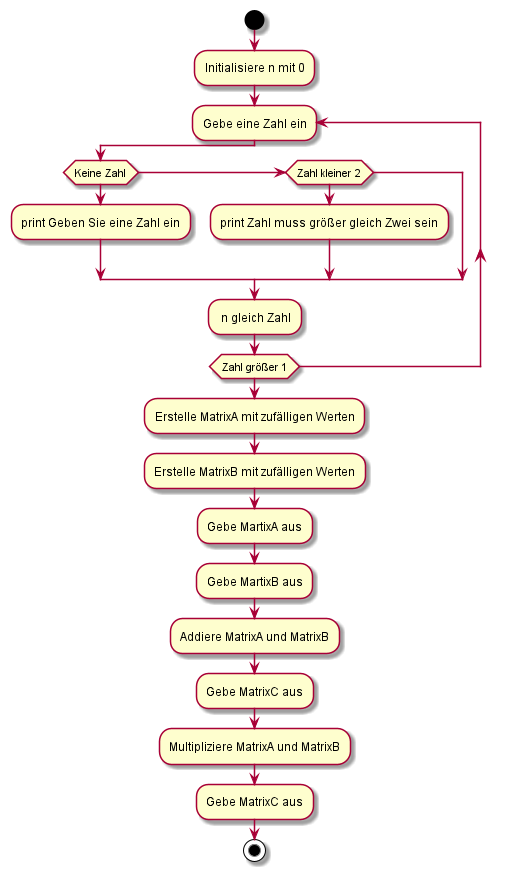
\includegraphics[scale=0.55]{uml/uml_c6_p1.png}

\subsubsection{Quelltext}
\paragraph{Matrizen.java}\
\lstinputlisting[language = Java , frame = trBL , escapeinside={(*@}{@*)}]{../chapter_06/src/chapter_06/Matrizen.java}

\subsubsection{Testdokumentation}
Bei Zahlen die kleiner als 2 waren, sowie Buchstaben, kam es zu einer entsprechenden Fehlermedlung. Anschließend konnte man den Wert erneut eintippen.

\subsubsection{Benutzungshinweise}
Nach dem aufrufen des Programmes, wird der nutzer aufgefordert eine Zahl einzugeben.
Diese muss grö\ss er als ein sein.

\subsubsection{Anwendungsbeispiel}
Nach dem man das Programm gestartet hat, sollte folgende Ausgabe erscheinen:
\begin{lstlisting}[frame = trBL , escapeinside={(*@}{@*)}]
[sebastian@laptop bin]$ java Matrizen 
Dieses Programm berechnet eine zufällig erstellte nxn Matrix
Geben sie n an: -45
Die Zahl muss größer gleich 2 sein
test
Es dürfen nur Zahlen verwendet werden
5
Matrix A:
78	88	96	91	50	
17	16	14	17	77	
34	1	45	21	42	
63	1	92	76	57	
84	59	13	85	46	

Matrix B:
38	36	45	22	18	
96	4	0	93	79	
86	38	92	50	92	
1	54	63	71	10	
4	62	91	31	55	

Addition von A und B:
116	124	141	113	68	
113	20	14	110	156	
120	39	137	71	134	
64	55	155	147	67	
88	121	104	116	101	

Multiplikation von A und B:
For Schleife
19959	14822	22625	22711	20848	
3711	6900	10131	6156	7263	
5447	6676	10815	5884	7351	
10706	13406	21274	13242	13572	
10243	11196	14517	15446	10749	

While Schleife
19959	14822	22625	22711	20848	
3711	6900	10131	6156	7263	
5447	6676	10815	5884	7351	
10706	13406	21274	13242	13572	
10243	11196	14517	15446	10749	

Do-While Schleife
19959	14822	22625	22711	20848	
3711	6900	10131	6156	7263	
5447	6676	10815	5884	7351	
10706	13406	21274	13242	13572	
10243	11196	14517	15446	10749
[sebastian@laptop bin]$ 
\end{lstlisting}
\subsection{Teilaufgabe 2}
\subsubsection{Aufgabenstellung}
In der zweiten Teilaufgabe sollten wir ein Programm schreiben welches Sprunganweisungen in Java
 Sinnvoll verdeutlichen.

\subsubsection{Anforderungsdefinition}
\begin{enumerate}
	\item Verwendung von Sprunganweisungen.
	\item Mindestens ein switch-Anweisung.
\end{enumerate}

\subsubsection{Entwurf}
Im folgenden ist ein Entwurf für ein einfaches Login. Zuerst wird der Nutzer aufgefordert seine ID
anzugeben. Dabei wird geprüft ob es sich um eine Zahl handelt und ob diese Zahl grö\ss er gleich Eins ist.
Anschlie\ss end wird wird in einem switch überprüft ob eine solche ID existiert und ob das angegebene
Passwort auch das richtige ist. Wenn alles Stimmt wird eine Willkommens Nachricht  ausgegeben.
Andernfalls wird der Nutzer aufgefordert alles erneut einzutippen.
\begin{center}
	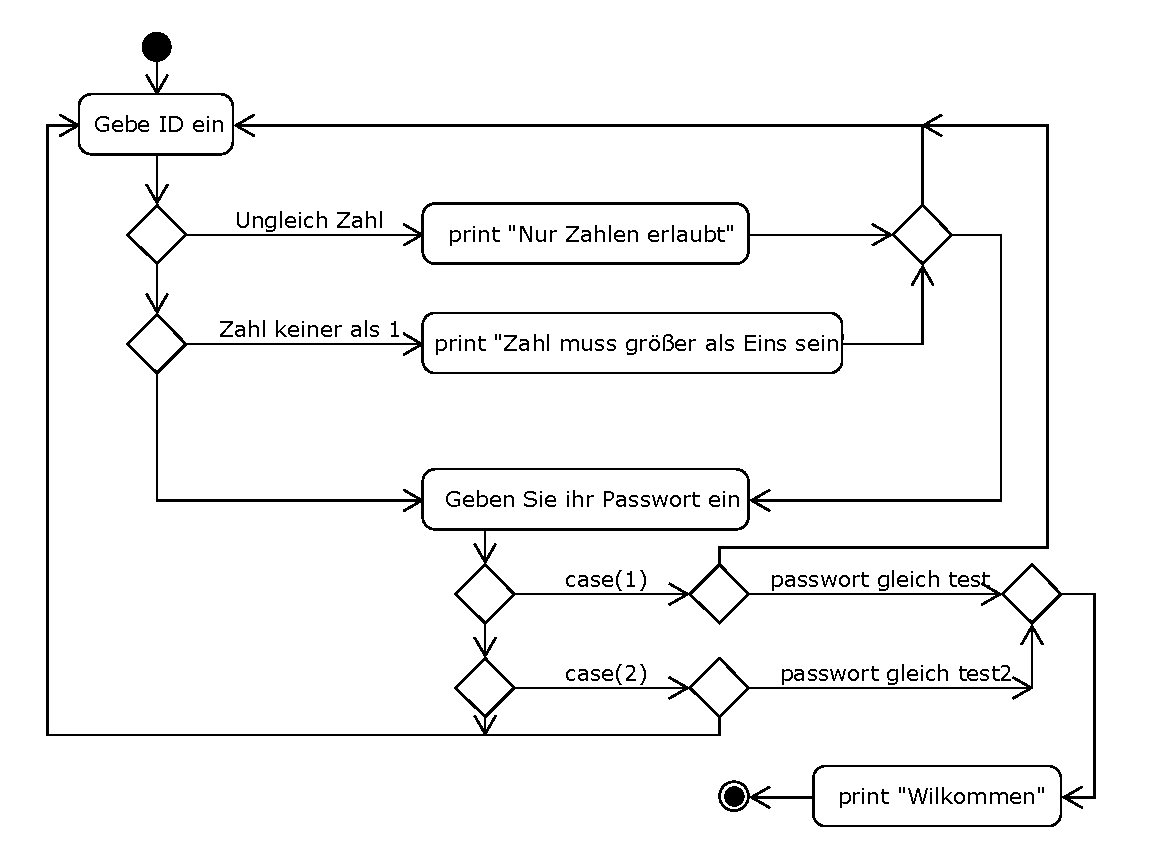
\includegraphics[width=0.8\textwidth]{uml/uml_c6_p2.pdf}
\end{center}

\subsubsection{Quelltext}
\paragraph{Sprunganweisungen.java}\
\lstinputlisting[language = Java , frame = trBL , escapeinside={(*@}{@*)}]{../chapter_06/src/main/java/chapter_06/Sprunganweisungen.java}

\subsubsection{Testdokumentation}
Bei Zahlen die kleiner als 1 waren, sowie Buchstaben, kam es zu einer entsprechenden Fehlermeldung. Anschlie\ss end konnte man den Wert erneut eintippen.

\subsubsection{Benutzungshinweise}
Nach dem aufrufen des Programms, wird der Nutzer aufgefordert seine NutzerID anzugeben,
sowie anschlie\ss end sein Passwort. Bei inkorrekter eingaben, wird man erneut aufgefordert
die Daten einzutippen.

\subsubsection{Anwendungsbeispiel}
Bei Erfolgreicher Anmeldung:
\begin{lstlisting}[frame = trBL , escapeinside={(*@}{@*)}]
[sebastian@laptop bin]$ java Sprunganweisungen 	
Wilkommen...!
ID      : 1
Passwort: hallo
Juhu, Sie haben sich eingeloggt
[sebastian@laptop bin]$ 
\end{lstlisting}
Bei inkorrekter Anmeldung:
\begin{lstlisting}[frame = trBL , escapeinside={(*@}{@*)}]
[sebastian@laptop bin]$ java Sprunganweisungen 	
Wilkommen...!
ID      : 12
Passwort: qwert
Ihre Angaben sind leider falsch, versuchen Sie es erneut.
ID      : -1
Passwort: hallo
Die Zahl muss größ er gleich 1 sein
ID      : 
[sebastian@laptop bin]$ 
\end{lstlisting}
\section{Kapitel 7}
\subsection{Aufgabenstellung}
Wie sollen 7 Klassen Definieren, dabei sollen wir uns überlegen welche davon Instanziierbar sind und welche
nicht. Anschließen soll jede Klasse sinnvolle Methoden und Attribute enthalten.

\subsection{Anforderungsdefinition}
\begin{enumerate}
	\item Definiere folgende Klassen: Viereck, konvexes Viereck, Trapez, Parallelogramm, Rhombus, Rechteck, Quadrat
	\item Definiere sinnvolle Methoden und Attribute
\end{enumerate}

\subsection{Entwurf}
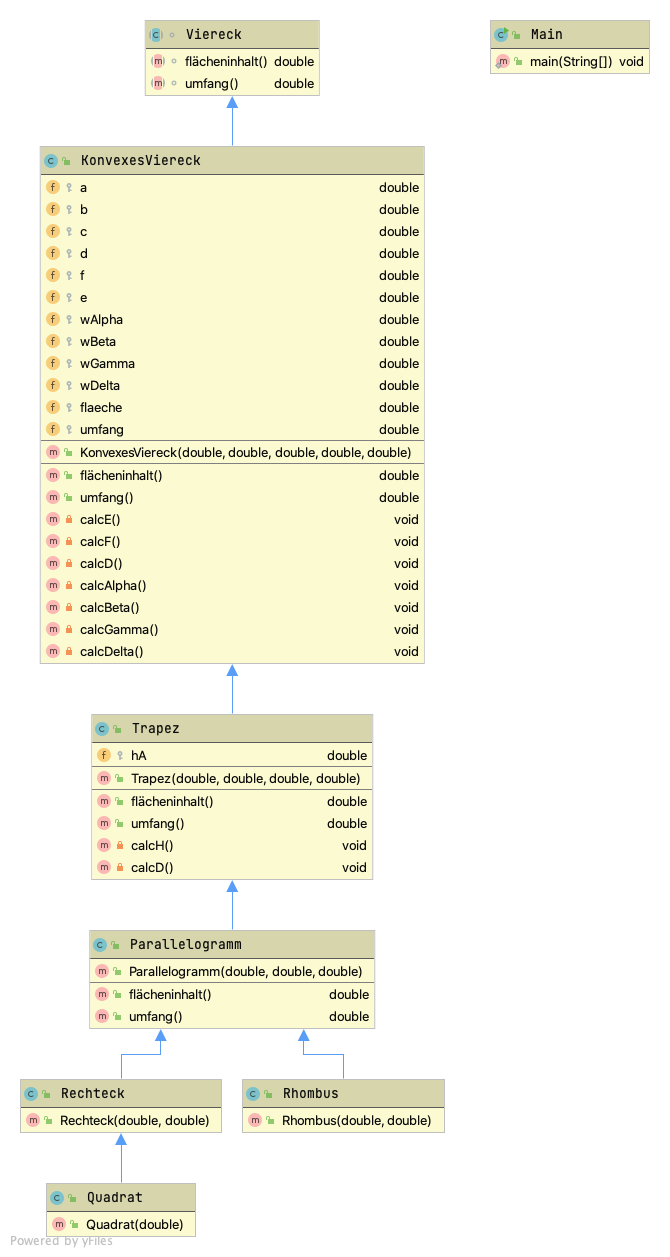
\includegraphics[scale=0.55]{uml/uml_c7_p1.png}

\subsection{Quelltext}
\subsubsection{Main.java}\
\lstinputlisting[language = Java , frame = trBL , escapeinside={(*@}{@*)}]{../chapter_07/src/chapter_07/Main.java}
\subsubsection{Viereck.java}\
\lstinputlisting[language = Java , frame = trBL , escapeinside={(*@}{@*)}]{../chapter_07/src/chapter_07/figures/Viereck.java}
\subsubsection{KonvexesViereck.java}\
\lstinputlisting[language = Java , frame = trBL , escapeinside={(*@}{@*)}]{../chapter_07/src/chapter_07/figures/KonvexesViereck.java}
\subsubsection{Trapez.java}\
\lstinputlisting[language = Java , frame = trBL , escapeinside={(*@}{@*)}]{../chapter_07/src/chapter_07/figures/Trapez.java}
\subsubsection{Parallelogramm.java}\
\lstinputlisting[language = Java , frame = trBL , escapeinside={(*@}{@*)}]{../chapter_07/src/chapter_07/figures/Parallelogramm.java}
\subsubsection{Rhombus.java}\
\lstinputlisting[language = Java , frame = trBL , escapeinside={(*@}{@*)}]{../chapter_07/src/chapter_07/figures/Rhombus.java}
\subsubsection{Rechteck.java}\
\lstinputlisting[language = Java , frame = trBL , escapeinside={(*@}{@*)}]{../chapter_07/src/chapter_07/figures/Rechteck.java}
\subsubsection{Quadrat.java}\
\lstinputlisting[language = Java , frame = trBL , escapeinside={(*@}{@*)}]{../chapter_07/src/chapter_07/figures/Quadrat.java}

\subsection{Testdokumentation}
?

\subsection{Benutzungshinweise}
?

\subsection{Anwendungsbeispiel}
Nach dem man das Programm gestartet hat, sollte folgende Ausgabe erscheinen:
\begin{lstlisting}[frame = trBL , escapeinside={(*@}{@*)}]
	[sebastian@laptop bin]$ java Main
	20.0 50.0
	20.0 50.0
	20.0 15.0
	30.0 50.0
	20.0 25.0
	[sebastian@laptop bin]$ 
\end{lstlisting}
\section{Kapitel 8}
\subsection{Aufgabenstellung}
Wir sollen ein Klasse schreiben die Nur Gerade zahlen annimmt, andernfalls soll eine Exception
geworfen werden. Zusätzlich kommen noch zwei Methoden in diese Klasse für 
die Multiplikation und Addition.

\subsection{Anforderungsdefinition}
\begin{enumerate}
	\item Erstelle eine Klasse GeradeZahl.
	\item Erstelle eine Methode für die Multiplikation und Addition.
	\item Bei ungeraden Zahlen soll eine Exception geworfen werden.
\end{enumerate}

\subsection{Entwurf}
\begin{center}
	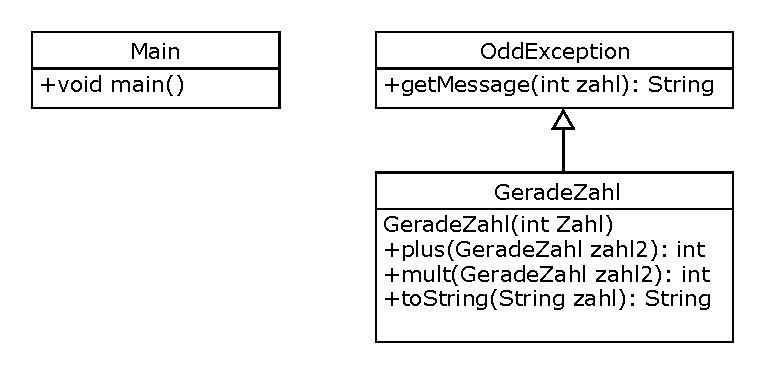
\includegraphics[width=0.99\textwidth]{uml/uml_c8_p1.pdf}
\end{center}

\subsection{Quelltext}
\subsubsection{Main.java}
\lstinputlisting[language = Java , frame = trBL , escapeinside={(*@}{@*)}]{../chapter_08/src/main/java/chapter_08/Main.java}
\subsubsection{GeradeZahl.java}
\lstinputlisting[language = Java , frame = trBL , escapeinside={(*@}{@*)}]{../chapter_08/src/main/java/chapter_08/GeradeZahl.java}
\subsubsection{OddException.java}
\lstinputlisting[language = Java , frame = trBL , escapeinside={(*@}{@*)}]{../chapter_08/src/main/java/chapter_08/OddException.java}

\subsection{Testdokumentation}
Bei einer Ungeraden Zahl wurde eine Exception geworfen und wie erwarte die Zahl
anschließend um eins erhöht.

\subsection{Benutzungshinweise}
Keine Besonderen Benutzungshinweise.
Das Programm muss lediglich nur ausgeführt werden.

\subsection{Anwendungsbeispiel}
Bei einer ungeraden Zahl sollte diese Ausgabe erscheinen.
\begin{lstlisting}[frame = trBL , escapeinside={(*@}{@*)}]
[sebastian@laptop bin]$ java Main
Exception in thread "main" chapter_08.OddException: Error, 21 ist keine Gerade Zahl! Die Zahl wurde um Eins erhöht.
at chapter_08.GeradeZahl.<init>(GeradeZahl.java:14)
at chapter_08.Main.main(Main.java:11)
[sebastian@laptop bin]$ 
\end{lstlisting}
Und bei einer Geraden diese.
\begin{lstlisting}[frame = trBL , escapeinside={(*@}{@*)}]
[sebastian@laptop bin]$ java Main
Zahl 1 = 200
Zahl 2 = 20
Zahl 3 = 600
Zahl 4 = 24
[sebastian@laptop bin]$ 
\end{lstlisting}
\section{Kapitel 10}
\subsection{Aufgabenstellung}
Wir sollen ein Programm schreiben Welches ein Artikel von der Tagesschau herunterlädt und
anschlie\ss end in einer Datei abspeichert. Der Nutzer kann angeben, welche Datei er einlesen möchte,
anschlie\ss end kann er die gezählten Wörter in Alphabetischer Reihenfolge ausgeben lassen.
Zusätzlich soll über ein Startparameter entschieden werden, ob Gro\ss -  und Kleinschreibung
beachtet wird.

\subsection{Anforderungsdefinition}
\begin{enumerate}
	\item Ein Artikel der Tagesschau mit mehr als 500 Wörtern soll runter geladen werden.
	\item Die Wörter sollen in einer geeigneten Collection abgelegt werden,
	\item Die Wörter sollen Sortiert ausgegeben können.
	\item Bei der Ausgabe der Wörte wird zusätzlich die Häufigkeit mit angegeben.
	\item Beim Start soll entschieden werden ob Gro\ss - oder Kleinschreibung.
\end{enumerate}

\subsection{Entwurf}
Zum Entwurf wurde ein Klassendiagramm gewählt welches die Methoden und deren Attribute der
jeweiligen Klassen veranschaulicht. DIe IO Klasse befasst sich mit dem Einlesen einer Datei, sowie auch
das anlegen neuer Dateien. Des weiterem kann die Klasse auch einen Artikel von der Tagesschau heruntergeladen werden, hierfür muss nur ein Link angegeben werden. Wenn ein Artikel heruntergeladen
wurden, kann dieser eingelesen werden und anschlie\ss end Sortiert ausgeben werden.
\begin{center}
	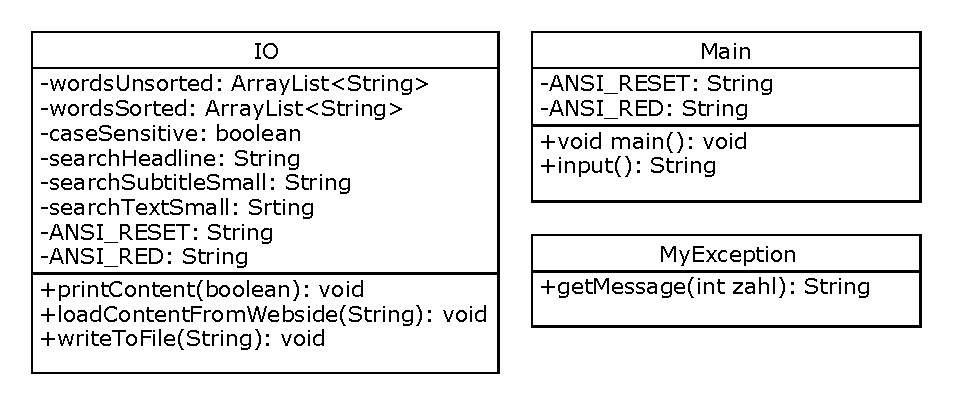
\includegraphics[width=0.98\textwidth]{uml/uml_c10_p1.pdf}
\end{center}

\subsection{Quelltext}
\subsubsection{Main.java}
\lstinputlisting[language = Java , frame = trBL , escapeinside={(*@}{@*)}]{../chapter_10/src/main/java/chapter_10/Main.java}
\subsubsection{IO.java}
\lstinputlisting[language = Java , frame = trBL , escapeinside={(*@}{@*)}]{../chapter_10/src/main/java/chapter_10/IO.java}
\subsubsection{MyException.java}
\lstinputlisting[language = Java , frame = trBL , escapeinside={(*@}{@*)}]{../chapter_10/src/main/java/chapter_10/MyException.java}

\subsection{Testdokumentation}
\begin{itemize}
	\item Startparameter:
	\subitem Bei einem inkorrekten Startparameter wird eine Exception geworfen.
	\item Menüauswahl:
	\subitem Bei falscher Eingabe wurde eine entsprechende Fehlermeldung ausgegeben.
	\item Artikel herunterladen:
	\subitem Wenn der Link nicht existiert kommt eine Fehlermeldung.
	\item Datei Laden:
	\subitem Wenn keine Datei gefunden wird mit den Namen kommt eine Fehlermeldung.
	\item Wörter ausgeben:
	\subitem Wenn keine Datei geladen wurde, kommt eine entsprechende Fehlermeldung.
\end{itemize}

\subsection{Benutzungshinweise}
Bei dem Aufruf des Programmes muss mit true oder false angegeben werden, ob Gro\ss - und
Kleinschreibung zu beachten ist. Anschlie\ss end kann man in dem Menü auswählen ob man einen
Artikel von der Tagesschau herunterladen möchte, eine Datei einlesen oder die Wörter in 
Alphabetischer Reihenfolge ausgibt.

\subsection{Anwendungsbeispiel}
\begin{lstlisting}[frame = trBL , escapeinside={(*@}{@*)}]
	[sebastian@laptop bin]$ java Main 	
	Exception in thread "main" chapter_10.MyException: Error, nur true oder false erlaubt
	at chapter_10.Main.main(Main.java:21)
	[sebastian@laptop bin]$ 
	[sebastian@laptop bin]$ java Main 
	Bitte wähle einer der Folgenden Optionen aus:
	1) Einen Artikel von der Tagesschau herunterladen.
	2) Eine Datei laden.
	3) Wörter ausgeben.
	0) Programm Beenden.
	1
	Bitte gebe den Link an:
	https://www.tagesschau.de/inland/gesellschaft/johnsonjohnson-103.html
	Loading Content
	Loading done
	Data written do file called: Warum punktet der neue Impfstoff.txt
	
	Bitte wähle einer der Folgenden Optionen aus:
	1) Einen Artikel von der Tagesschau herunterladen.
	2) Eine Datei laden.
	3) Wörter ausgeben.
	0) Programm Beenden.
	a
	Es sind nur Zahlen erlaubt
	b
	Es sind nur Zahlen erlaubt
	2
	Bitte geben Sie den Datei namen an:
	Warum punktet der neue Impfstoff
	Datei wurde Erfolgreich geladen
	
	Bitte wähle einer der Folgenden Optionen aus:
	1) Einen Artikel von der Tagesschau herunterladen.
	2) Eine Datei laden.
	3) Wörter ausgeben.
	0) Programm Beenden.
	3
	ab 4x
	aber 4x
	abgeschwaechten 1x
	aehnliche 1x
	aehnliches 1x
	aendern 1x
	Alle 2x
	allen 2x
	allerdings 1x
	Allergien 1x
	allergischen 1x
	als 2x
	also 1x
	alsoauch 1x
	Altersgruppe 1x
	am 1x
	amp 1x
	an 3x
	anderen 3x
	anhaelt 1x
	ansteckend 1x
	Antikoerper 2x
	Anwendung 1x
	Anzahl 1x
	Arzneimittel-Agentur 1x
	Arzneimittelhersteller 2x
	AstraZeneca 4x
	AstraZeneca-Impfstoff 1x
	Auch 3x
	auch 6x
	auf 2x
	aus 3x
	ausreichende 1x
	Ausserdem 1x
	basierte 1x
	bauen 1x
	Bauplan 2x
	Bei 8x
	bei 8x
	beide 1x
	beiden 1x
	bekommen 1x
	beobachteten 1x
	bereits 4x
	Berichte 1x
	Beschwerden 1x
	bildet 2x
	BioNTechPfizer 5x
	BioNTechPfizernbspbei 1x
	bisher 1x
	bisherigen 1x
	bleibt 1x
	Brasilien 2x
	britischen 1x
	Coronavirus 5x
	Coronavirus-Erbgutes 1x
	Dabei 1x
	dafuer 1x
	Damit 1x
	damit 3x
	Darauf 1x
	darauf 1x
	darueber 1x
	Das 4x
	das 5x
	dass 4x
	Datenlage 2x
	Dazu 1x
	dem 4x
	den 14x
	denen 1x
	denn 1x
	dennoch 1x
	Der 5x
	der 25x
	des 7x
	deuten 1x
	Deutschland 4x
	Die 3x
	die 23x
	dies 1x
	Diese 3x
	diese 1x
	direkt 1x
	Dort 1x
	dort 1x
	Dosis 1x
	drei 2x
	ebenfalls 1x
	ein 4x
	Ein-Mal-Dosis 1x
	eine 5x
	einen 3x
	einer 2x
	eines 1x
	eineSchutzwirkung 1x
	einfachen 1x
	eingeraeumt 1x
	Einschraenkung 1x
	Einstichstelle 1x
	Empfehlung 2x
	empfiehlt 1x
	empfindlicher 1x
	entscheidet 1x
	entsprechende 1x
	Entwicklung 1x
	er 1x
	Erbmaterials 1x
	Ergebnis 1x
	Ergebnisse 1x
	Ergebnissen 1x
	Erkrankungen 1x
	erreicht 1x
	Erste 1x
	ersten 2x
	es 5x
	etwas 1x
	EU-Arzneimittelbehoerde 1x
	Europaeische 1x
	Europageaendert 1x
	Exakte 1x
	Faellen 1x
	Fall 1x
	flaechendeckend 1x
	fuer 3x
	funktioniert 1x
	Gefrierschranktemperaturenstabil 1x
	gegeben 1x
	gegen 6x
	gegenueber 1x
	gehoeren 1x
	geimpft 6x
	Geimpfte 1x
	geimpfte 1x
	Geimpften 1x
	gelagert 1x
	Gelenkschmerzen 1x
	genau 1x
	generelle 1x
	genetische 2x
	geringer 1x
	geringeren 1x
	getestet 2x
	gibt 2x
	gleiche 1x
	Grad 2x
	groesseren 1x
	Grossbritannien 1x
	grosser 1x
	Grund 1x
	haeufigsten 1x
	haltbar 1x
	handelt 1x
	hat 7x
	hatteBioNTechbekannt 1x
	hatten 2x
	heisst 1x
	hier 1x
	hindass 1x
	hingegen 1x
	hoch 1x
	hohe 1x
	ihre 1x
	ihrer 1x
	im 2x
	Immunsystem 2x
	Impfdosis 1x
	impfen 1x
	Impfkommission 2x
	Impfstoff 11x
	Impfstoffe 4x
	Impfstoffen 3x
	Impfstoffs 1x
	Impfung 4x
	In 3x
	in 20x
	Infektionen 1x
	Information 1x
	Inhaltsstoffe 1x
	Israel 1x
	ist 11x
	Jaehrige 1x
	Jahren 4x
	jeden 1x
	Johnson 18x
	kam 1x
	keine 1x
	klangen 1x
	klinischen 2x
	Koch-Institut 1x
	koennen 2x
	koennte 1x
	Koerper 1x
	kommenden 1x
	konnten 1x
	Kopf- 1x
	Kuehlschranktemperaturen 1x
	Laendern 1x
	lag 2x
	Lagerung 1x
	lange 3x
	lassen 1x
	laufen 2x
	laut 2x
	liegen 1x
	Mal 2x
	manche 1x
	mehrere 1x
	mehreren 1x
	meisten 1x
	Menschen 6x
	menschliche 1x
	Minus 2x
	Minusgraden 1x
	mit 5x
	mithilfe 1x
	Moderna 6x
	Monaten 1x
	mRNA-Impfstoffen 2x
	Muedigkeit 1x
	muessen 1x
	muss 1x
	Mutation 1x
	Mutationen 2x
	mutierten 1x
	nach 3x
	nachgebaut 1x
	Nachteile 1x
	neben 1x
	Nebenwirkungen 2x
	neuartigen 1x
	neue 2x
	nicht 4x
	niedriger 1x
	noch 4x
	noetig 1x
	normalen 2x
	Notfallzulassung 1x
	Nun 1x
	Nur 1x
	nur 4x
	Ob 1x
	ob 1x
	Oberflaechenproteine 1x
	ObTransport 1x
	oder 4x
	Personen 1x
	Praeparat 2x
	Praeparate 1x
	Praeparats 1x
	Prioritaet 1x
	Probanden 2x
	Prozent 6x
	pruefen 1x
	punktet 1x
	reagiert 2x
	Reaktionen 1x
	RKI 1x
	Robert 1x
	schaedlich 1x
	Schmerzen 1x
	schnell 1x
	Schuettelfrost 1x
	schuetzen 1x
	schuetzt 1x
	Schutz 1x
	Schutzwirkung 3x
	Schwere 1x
	schwere 1x
	schweren 1x
	sehr 1x
	sein 1x
	sich 6x
	Sicht 1x
	sie 2x
	sind 7x
	so 1x
	sogenannten 1x
	soll 1x
	sollten 1x
	sondern 1x
	Staendigen 1x
	StiKo 2x
	Studien 5x
	Studienvorliegen 1x
	Suedafrika 3x
	suedafrikanischen 1x
	Symptomen 1x
	tatsaechlich 1x
	Teil 1x
	Teile 2x
	Teils 1x
	Todesfaelle 1x
	Traegerviren 1x
	Traegervirus 2x
	transportiert 1x
	trotz 1x
	ueber 1x
	uebertragen 1x
	um 1x
	und 15x
	ungefaehrlich 1x
	Unklar 1x
	unklar 1x
	Unternehmen 1x
	unterschiedliche 1x
	untersucht 1x
	Untersuchungen 1x
	urspruengliche 1x
	USA 1x
	Variante 1x
	Varianten 1x
	Vektorimpfstoff 1x
	VektorimpfstoffenbspDas 1x
	verbessert 1x
	Vergleich 1x
	vergleichbar 1x
	verhindert 1x
	verimpft 2x
	Verlaeufe 1x
	verpackt 1x
	Vertraeglichkeit 1x
	verwenden 1x
	viele 1x
	Vier 1x
	vier 2x
	Viren 2x
	Virus 1x
	von 21x
	vor 2x
	Vor- 1x
	Vorteil 2x
	Vorteile 1x
	war 1x
	Warum 1x
	weitertragen 1x
	Welche 3x
	welche 1x
	Welcher 1x
	wenigen 1x
	weniger 2x
	wenn 2x
	werden 8x
	Wie 3x
	wie 6x
	wieder 1x
	wird 4x
	Wirken 1x
	wirksam 1x
	Wirksamkeit 4x
	Wirkstoffe 1x
	wirkt 1x
	Wirkungsweise 1x
	wo 1x
	Wochen 2x
	worden 2x
	wurde 3x
	Zahlen 1x
	zeigen 2x
	zeigte 1x
	Zelle 1x
	Zellen 1x
	Zu 1x
	zu 3x
	zudem 1x
	zufolge 2x
	zugelassen 1x
	zugelassenen 2x
	zunaechst 1x
	zurueckgenommenNun 1x
	Zusammenhang 1x
	zwei 1x
	zweiten 1x
	Bitte wähle einer der Folgenden Optionen aus:
	1) Einen Artikel von der Tagesschau herunterladen.
	2) Eine Datei laden.
	3) Wörter ausgeben.
	0) Programm Beenden.
	0
	[sebastian@laptop bin]$ 
\end{lstlisting}

\printbibliography

%%% Protokoll: Ende
\end{document}